
%%%%%%%%%%%
%remove tag+probe ref
%%%%%%%%%%%


\subsection{Opposite Flavor Subtraction}
\label{sec:ofsub}


{\bf this section is a place holder for Niklas to put in his stuff}

With much more statistics, we could also use an opposite-flavor subtraction
technique which takes advantage of the fact that the ttbar yield in the opposite-flavor final state ($e\mu$) is the same as in the same-flavor final state
($ee+\mu\mu$), modulo differences in efficiency in the $e$ vs.\ $\mu$ selection. Hence the ttbar yield in the same-flavor final state can be estimated
using the corresponding yield in the opposite-flavor final state. The simplest option is to take the $e\mu$ yield inside the $Z$ mass window and scale this
to predict the $ee$ and $\mu\mu$ yields, based on $e$ and $\mu$ selection efficiencies.
Only the ratio of electron to muon selection efficiency is needed, which we evaluate as $\epsilon_{\mu e} = \sqrt{\frac{N_{Z\mu\mu}}{N_{Zee}}}$. 
Here $N_{Zee}$ ($N_{Z\mu\mu}$) is the total number of events in the $ee$ ($\mu\mu$) final state passing the pre-selection in Section~\ref{sec:yields},
with the requirement of at least 2 jets removed. We find $\epsilon_{\mu e}=1.06 \pm 0.01$ (note that in the following $\epsilon_{e\mu} = 1/\epsilon_{\mu e}$, and the error on the efficiency ratio is statistical).

This procedure yields the following predicted yields $n_{pred}$, based on an observed yield of 2 $e\mu$ events in the signal region:

\begin{equation}
%my results for 11/pb
n_{pred}(\mu\mu) = \frac{1}{2}n(e\mu)\epsilon_{\mu e} = 1.1 \pm 0.8 \pm x
%prev number for 30/pb: 3.6 \pm 1.4~(stat) \pm 0.2~(syst)
\end{equation}
\begin{equation}
n_{pred}(ee)     = \frac{1}{2}n(e\mu)\epsilon_{e\mu} = 0.94 \pm 0.7 \pm x
%prev : = 2.9 \pm 1.2~(stat) \pm 0.1~(syst).
\end{equation}

%I find this unclear, so I will try to reword it
%The predicted yields agree well with the observed yields of 2.7 ($ee$) and 3.5 ($\mu\mu$) as shown in Fig.~\ref{fig:ttbar}. 
The predicted same flavor ttbar yields agree well with the MC expectation of 1.03 ($\mu\mu$) %really 1.03244
and 1.0 ($ee$) %really 1.00441385
as shown in Fig.~\ref{fig:ttbar}. %plot to be updated
Due to the small statistics, the errors on the predicted yields using this procedure are quite large.
To improve the statistical errors, we instead determine the $e\mu$ yield without requiring the leptons to fall in the $Z$ mass window. 
This yield is scaled by a factor determined from MC, $K$ (0.236 $\pm x$) %(0.225) 
which accounts for the fraction of ttbar events expected to fall in the $Z$ mass window. This procedure yields the following
predicted yields based on 8 observed $e\mu$ events:

\begin{equation}
n_{pred}(\mu\mu) = \frac{1}{2}n(e\mu)K\epsilon_{\mu e} = 1.0 \pm 0.4 \pm x
%n_{pred}(\mu\mu) = n(e\mu)/8.0 = 3.6 \pm 0.7~(stat) \pm 0.4~(syst)
\end{equation}
\begin{equation}
n_{pred}(ee)     = \frac{1}{2}n(e\mu)K\epsilon_{e\mu} = 0.89 \pm 0.3 \pm x
%n_{pred}(ee)     = n(e\mu)/9.8 = 3.0 \pm 0.5~(stat) \pm 0.3~(syst).
\end{equation}

Notice that the statistical uncertainty is reduced by a factor of approximately 2, while we are currently assessing the systematic uncertainties.
Since the total uncertainty is expected to be statistically-dominated, the second method yields a better prediction and we use this as our estimate
of the \ttbar~background.


\begin{figure}[hbt]
  \begin{center}
    \resizebox{0.75\linewidth}{!}{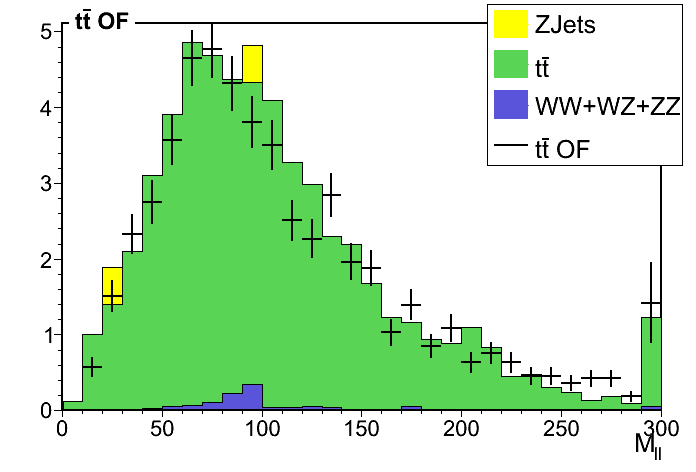
\includegraphics{flavorsubdata.png}}
    \caption{Dilepton mass distribution for events passing the signal region selection. The solid histograms represent the yields in the same-flavor
      final state for each SM contribution, while the solid black line (OFOS) indicates the sum of the MC contributions in the opposite-flavor final state.
      %The observed ttbar yields inside the $Z$ mass window in the $ee$ and $\mu\mu$ final states are indicated. 
      The ttbar distribution in the same-flavor final state is well-modeled by the OFOS prediction.}
    \label{fig:ttbar}
  \end{center}
\end{figure}
